\paragraph{Scenarios}
    \begin{enumerate}
        \item Johnny is a model citizen of Milan and he is really caring about parking violations, because they are really recurrent in his neighbourhood. When he see a violation, he open the SafeStreets app on his smartphone and report it with just few clicks. All he needs to do is to take a photo of the violation where the licence plate is clearly visible and confirm if the system detected it correctly or not, if not he insert the licence plate manually in the field that appears after the confirmation. Position is automatically detected from the GPS because he allowed the app to access it, and to send the report to SafeStreets he just need to confirm by clicking the done button.
    \end{enumerate}

\begin{figure}[htbp]
	\centering
    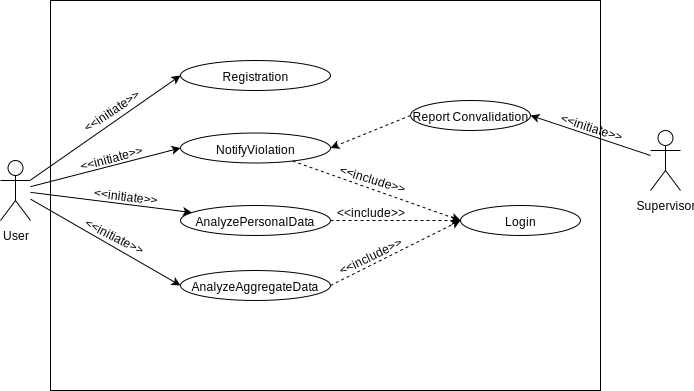
\includegraphics[width=\textwidth]{Images/UseCaseUser}
\end{figure}	
\textbf{Use cases}\\
\vskip 0.2in

\begin{tabular}{|p{3.7cm}|p{11cm}|}
\hline
Name & NotifyViolations\\
\hline
Actors & Citizen\\
\hline
Entry Condition & Violation detection.\\
\hline
Event flow & \begin{enumerate}
                \item The User selects the report tab if not already selected.
                \item The User selects the type of violation.
                \item The User takes and uploads a photo of the violation.
                \item The User confirms that the license plate is correctly recognised by app, if not he/she inserts it manually in the appropriate field.
                \item The User checks whether his/her current position is correctly identified by the GPS system, if not he/she inserts it manually in the appropriate field.
                \item The User confirms the violation report clicking on the "Done" button.
                \item The system stores the information and completes it with suitable metadata.
                \item The system sends a notification to the User about the success of the operation.
            \end{enumerate}\\
\hline
Exit condition & The violation report is correctly stored.\\
\hline
Exception & the system detects missing information and rejects the report, then asks the User for missing data.\\
\hline
Special requirement & TBD.\\
\hline
\end{tabular}

\vskip 0.2in
\begin{tabular}{|p{3.7cm}|p{11cm}|}
\hline
Name & AnalyzeAggregateData\\
\hline
Actors & Citizen\\
\hline
Entry Condition & The Actor wants to know some information about the reported violations.\\
\hline
Event flow & \begin{enumerate}
                \item The Actor selects the "aggregated data" tab.
                \item The Actor selects the topic he/she is interested about.
                \item The Actor may select an appropriate filter for his search.
                \item The Actor selects the data of interest.
                \item The system provides the data to be visualized according to the actor's authorization level.
                \item The Actor visualizes the data.
            \end{enumerate}\\
\hline
Exit condition & The Actor finishes to analyze the data.\\
\hline
\end{tabular}

\vskip 0.2in
\begin{tabular}{|p{3.7cm}|p{11cm}|}
\hline
Name & Login\\
\hline
Actors & Citizen\\
\hline
Entry Condition & The actor opens the app.\\
\hline
Event flow & \begin{enumerate}
                \item The actor inserts his username.
                \item The actor inserts his password.
                \item The actor press the login button.
            \end{enumerate}\\
\hline
Exit condition & The actor is authenticated and login is successful.\\
\hline
Exception & Username or password are invalid, "invalid credential" message is displayed and the actor needs to insert credential again.\\
\hline
\end{tabular}

\vskip 0.2in
\begin{tabular}{|p{3.7cm}|p{11cm}|}
\hline
Name & UserRegistration\\
\hline
Actors & Citizen\\
\hline
Entry Condition & The user opens the app and has no valid account.\\
\hline
Event flow & \begin{enumerate}
                \item The user inserts the desired username.
                \item The user inserts the desired password.
                \item The user confirms his password.
                \item The user inserts his email.
                \item The user inserts his birthday.
                \item The user agrees to the use of his personal data and of his submitted violation reports for analysis purposes.
            \end{enumerate}\\
\hline
Exit condition & The registration is successful and the user is redirected to login form.\\
\hline
Exception & Email is already in use or confirm password field content diverge from password, in this case the user is alerted with a proper message on screen and asked to correct the data.\\
\hline
\end{tabular}